% !TEX options=--shell-escape
\documentclass[usenames,dvipsnames,9pt]{beamer}

\usepackage{tikz}
\usetikzlibrary{arrows,shapes,snakes,automata,calc,matrix,backgrounds,petri, positioning}

\makeatletter
\def\input@path{{support/beamer-template/}}
\makeatother

\usepackage{support/beamer-template/beamerthememetropolis}

\usepackage[utf8]{inputenc}
\usepackage[czech]{babel}
\selectlanguage{czech}

\usepackage{hyperref}
\usepackage{fontawesome}
\usepackage{minted}
\usepackage{mathtools}
\usepackage{tabularx}
\usepackage{smartdiagram}
\usepackage{soul}
\usepackage{tikz}
\usepackage{amssymb}
\usepackage{qrcode}

% Commands shared between most of the tutorial slides

% Homework deadlines
\newcommand{\hwVIIdeadline}{10. 5. 2020}



% Download icon and text with link relative to the root of the courseware site
\newcommand{\download}[1]{\hfill\faDownload\hspace{5pt}\href{https://cw.fel.cvut.cz/wiki/_media/courses/be4m36mas/#1}{\tt #1}\\[1.3em]}

% Draw eye icon
\newcommand{\see}[1]{\faEye\hspace{5pt}#1}

\newcommand{\sep}{\hspace{10pt}/\hspace{10pt}}

\def\Ipe#1{\def\IPEfile{#1}\input{#1}}

% Draw pacman icon
\newcommand{\pacman}[1]{\tikz[baseline=.1em,scale=.6]{
    \useasboundingbox (.02,0) rectangle (.6,.6);
  \draw [fill=#1] (.3,.3) -- ++(25:.3) arc (+25:+335:.3) -- cycle;

}}

% Draw ghost icon
\newcommand{\ghost}[1]{\tikz[baseline=.1em,scale=.5]{
  \draw [fill=#1] (0,0) -- (0,.5) arc (+180:0:.3) -- (.6,0) --
  (.5,.15) -- (.4,0) -- (.3,.15) -- (.2,0) -- (.1,.15) -- cycle;
    \coordinate (eye) at (360*rand:.03);
    \foreach \x in {.17,.43}{
      \fill[white] (\x,.5) circle[radius=.1];
      \fill[black] (\x,.5) ++(eye) circle[radius=.05];
    }
}}

\newcommand{\desc}[2]{
  #1

  \vspace{-0.6em}
  \hfill\begin{minipage}{0.9\linewidth}
    #2
  \end{minipage}

  \vspace{0.2em}
}

\newcommand{\redc}{\tikz\draw[red,fill=red] (0,0) circle (.5ex);}

\newcommand{\greenc}{\tikz\draw[green,fill=green] (0,0) circle (.5ex);}


% Default url for generating QR code with feedback form.
\newcommand{\defaultfeedbackurl}{https://forms.gle/vwbWazEu14w1Kf487}

% Generate frame with QR code to a feedback form.
\newcommand{\framefeedback}[1][\defaultfeedbackurl]{
  \begin{frame}[standout]
    \begin{minipage}{0.4\linewidth}
      \begin{center}
        \textbf{\LARGE Díky za pozornost!}
      \end{center}

      \vspace{3em}

      \raggedleft\small Budeme rádi za Vaši\\zpětnou vazbu! $\rightarrow$
    \end{minipage}
    \hfill
    \begin{minipage}{0.5\linewidth}
      \vspace{4em}
      \centering\qrcode[height=\linewidth]{#1}\\
      \vspace{0.8em}
      \url{#1}
    \end{minipage}
  \end{frame}
}


% \newcommand{\download}[1]{\hfill\faDownload\hspace{5pt}\href{https://cw.fel.cvut.cz/wiki/_media/courses/be4m36mas/#1}{\tt #1}\\[1.3em]}
% \newcommand{\see}[1]{\faEye\hspace{5pt}#1}
% \newcommand{\sep}{\hspace{10pt}/\hspace{10pt}}
% \def\Ipe#1{\def\IPEfile{#1}\input{#1}}
%
% \newcommand{\pacman}[1]{\tikz[baseline=.1em,scale=.6]{
%     \useasboundingbox (.02,0) rectangle (.6,.6);
%   \draw [fill=#1] (.3,.3) -- ++(25:.3) arc (+25:+335:.3) -- cycle;
%
% }}
%
% \newcommand{\ghost}[1]{\tikz[baseline=.1em,scale=.5]{
%   \draw [fill=#1] (0,0) -- (0,.5) arc (+180:0:.3) -- (.6,0) --
%   (.5,.15) -- (.4,0) -- (.3,.15) -- (.2,0) -- (.1,.15) -- cycle;
%     \coordinate (eye) at (360*rand:.03);
%     \foreach \x in {.17,.43}{
%       \fill[white] (\x,.5) circle[radius=.1];
%       \fill[black] (\x,.5) ++(eye) circle[radius=.05];
%     }
% }}
%
%
% \newcommand{\desc}[2]{
%   #1
%
%   \vspace{-0.6em}
%   \hfill\begin{minipage}{0.9\linewidth}
%     #2
%   \end{minipage}
%
%   \vspace{0.2em}
% }
%
% \newcommand{\redc}{\tikz\draw[red,fill=red] (0,0) circle (.5ex);}
% \newcommand{\greenc}{\tikz\draw[green,fill=green] (0,0) circle (.5ex);}

\title{Konsenzus v distribuovaném systému}
\date{}
\institute{B4B36PDV -- Paralelní a distribuované výpočty}

\metroset{block=fill}

\begin{document}
\maketitle

\begin{frame}
  \frametitle{Osnova}
  \begin{itemize}
    \item Opakování z minulého cvičení\\[1.5em]
    \item Proč bychom mohli chtít řešit konsenzus v DS?
    \item RAFT algoritmus\\[1.5em]
    \item Zadání semestrální úlohy
  \end{itemize}
\end{frame}


\section{Opakování z minulého cvičení}

\begin{frame}[standout]
 \Huge
 \url{http://goo.gl/a6BEMb}
\end{frame}

%\begin{frame}
%\frametitle{DSand framework}
%\centering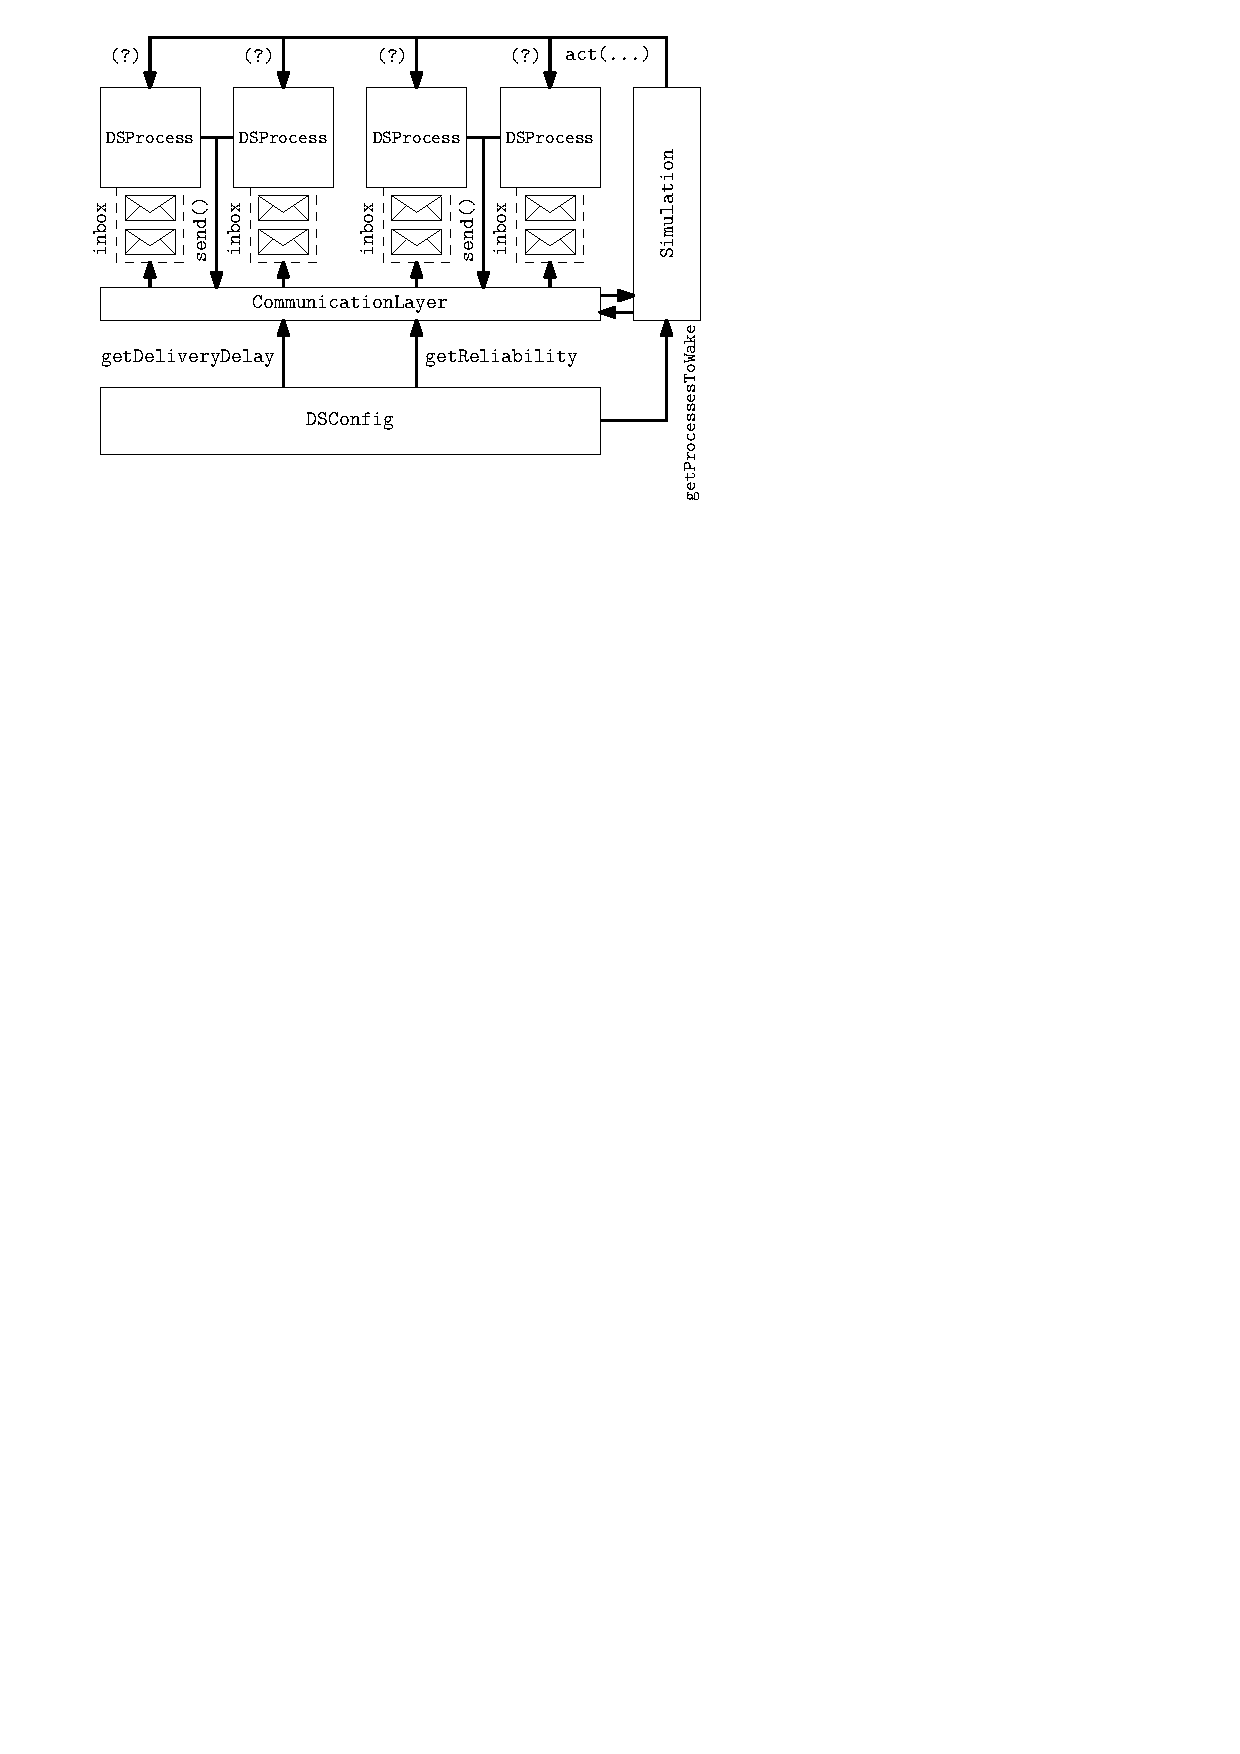
\includegraphics[width=0.8\linewidth]{12/figs/dsand.pdf}
%\end{frame}

{\setbeamertemplate{frame footer}{\see{\url{http://goo.gl/a6BEMb}}}
  \begin{frame}[fragile]
  \frametitle{Jaké vlastnosti mají vektorové hodiny?}
  \begin{enumerate}
  \item jsou paměťově náročnější než skal\'arn\'i hodiny \uncover<2->{- \textcolor{green}{TRUE}}
  \item dokáží detekovat porušení kauzality vůči konkrétnímu procesu \uncover<3->{- \textcolor{green}{TRUE}}
  \item generují částečné uspořádání zpráv \uncover<4->{- \textcolor{green}{TRUE}}
  \item určují reálný čas, kdy byla zpráva poslána \uncover<5->{- \textcolor{red}{FALSE}}
  \item dokáží detekovat, zda je daná událost kauzálním důsledkem jiné události \uncover<6->{- \textcolor{red}{FALSE}}
  \end{enumerate}
  \begin{overprint}[\textwidth]
    \onslide<3> Ano, vektorové hodiny správně zdetekují porušení kauzaility vždy.
    \onslide<4> Ano, všechny dvojice událostí jsou ve vztahu "nastalo po" nebo "je současné"
    \onslide<6> Hodiny nedokáží detekovat kauzalitu (následek nastal v důsledku příčiny), ale dokáží detekovat potenciální kauzalitu (následek mohl nastat v důsledku příčiny, tzn. existuje kauzální cesta od příčiny k následku)
  \end{overprint}
  \end{frame}


  \begin{frame}[fragile]
  \frametitle{Které z následujících algoritmů distribuovaného vzájemného vyloučení jsou férové?}
  \begin{enumerate}
  \item Centrální server \uncover<2->{- \textcolor{red}{FALSE}}
  \item Kruhové splňování \uncover<3->{- \textcolor{red}{FALSE}}
  \item Ricart-Agrawalovo vyloučení \uncover<4->{- \textcolor{green}{TRUE}}
  \end{enumerate}
  \vspace{2em}
  \begin{overprint}[\textwidth]
    % Férovost: "procesy získávají přístup k pořadí, v jakém o něj požádali"
    \onslide<2> Není splňen požadavek zachování pořadí, latence může změnit pořadí.
    \onslide<3> Není splňen požadavek zachování pořadí, pořadí dané pozicí v kruhu.
  \end{overprint}
  \end{frame}


  \begin{frame}[fragile]
  \frametitle{Který z následujících algoritmů distribuovaného vzájemného vyloučení je nejefektivnější z hlediska počtu poslaných zpráv?}
  \begin{enumerate}
    \item Centrální server \uncover<2->{- 3}
    \item Kruhové splňování \uncover<3->{- od 0 do n}
    \item Ricart-Agrawalovo vyloučení \uncover<4->{- 2(n-1)}
  \end{enumerate}
  \vspace{2em}
  \begin{overprint}[\textwidth]
    \onslide<2> Ale centrální server je "single point of failure".
    \onslide<3> Token koluje i když nikdo přístup do kritické sekce nepotřebuje, vysoké synchronizační zpoždění, tzn. čas mezi přístupy dvou po sobě jdoucích procesů do kritické sekce (O(n)).
  \end{overprint}
  \end{frame}

}

\section{Konsenzus v distribuovaném světě}

\begin{frame}
  \frametitle{Distribuovaná databáze}

  {\large Uvažujme upravený protokol, kdy klient čeká na potvrzení zápisu...}

  \begin{center}
    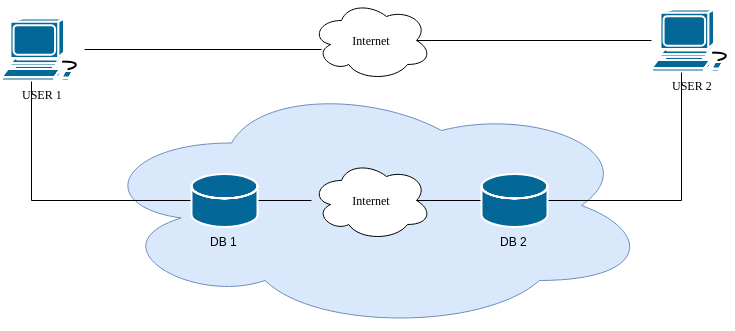
\includegraphics[width=0.8\linewidth]{12/figs/pdv_cloud.png}
  \end{center}

  \pause
  \begin{center}
    \Large Co se stane, když server zodpovědný za replikaci selže?
  \end{center}
\end{frame}

\begin{frame}
  \frametitle{Distribuovaná databáze}

  {\large\bf
    \begin{itemize}
      \item[\faWarning] Některé servery mohou znát aktuální data a jiné nikoliv!

                        \hfill {\normalfont\Large Potřebujeme se shodnout na společné ,,pravdě``} \\[2em]

      \pause
      \item[\faWarning] Zároveň se nám nesmí ztrácet data, o kterých si klient myslí, že jsou uložená
    \end{itemize}
  }
\end{frame}

\begin{frame}
  \frametitle{Jak to řeší centralizované databáze?}

  {\large Ukládání obsahu databáze na disk při každé operaci je drahé...}

  \hfill {\large \faWarning \hspace{3pt} Části databáze si proto raději držíme v paměti}

  \pause\vspace{3em}\hrule\vspace{0.2em}
  \begin{center}
    \LARGE Co když nám server po potvrzení zápisu spadne?
  \end{center}

  \vspace{1em}\pause
  {\large
    \textbf{Řešení:} Před potvrzením zápisu požadavek uložíme do logu (žurnálu\footnote{do zvláštní sekce disku nebo jiného perzistentního úložiště})!

    \hspace{20pt} $\rightarrow$ Pokud server spadne, z žurnálu obnovíme ztracená data

    \vspace{1em}

    Tomu se říká \emph{journaling} nebo \emph{write-ahead logging} a je součástí většiny ,,rozumných`` databázových systémů.
  }
\end{frame}

\begin{frame}
  \frametitle{Journaling v distribuované databázi}
  \begin{center}
    \LARGE Jak bychom mohli použít journaling v distribuované DB?
  \end{center}

  \pause
  \vspace{2em}\hrule\vspace{2em}

  {\Large Nemusíme se shodovat na konkrétním obsahu databáze} \\
  (ten může být potenciálně obrovský!)

  \vspace{1em}

  {\Large Stačí, když se shodneme na obsahu žurnálu} \\
  (a doplníme případné chybějící požadavky/záznamy)
\end{frame}

\section{Raft algoritmus}

\begin{frame}
  \frametitle{Raft}

  \begin{columns}
    \begin{column}{0.7\textwidth}
      \begin{center}
        \LARGE Algoritmus pro distribuovanou replikaci logů (koncenzus)
      \end{center}
    \end{column}
    \begin{column}{0.3\textwidth}
        \begin{center}
        
\includegraphics[width=0.8\textwidth]{12/figs/raft_logo.png}
        \end{center}
    \end{column}
  \end{columns}

  \uncover<2->{
      Cíle:
      \begin{itemize}
        \item Jednoduchost na pochopení 
        \item Úplnost a použitelnost (pokud je naimplementován tak funguje) 
      \end{itemize}  
      % Má stejné paramtery jako Paxos, ale je pochopitelnější.
    }
  \vspace{1em}
  \uncover<3->{
      Optimalizovaná verze použitá např. v MongoDB\footnote<3->{\href{https://henrikingo.github.io/presentations/PGDay\%20Russia\%202017\%20-\%20MongoDB\%20and\%20Raft/\#/title}{Slides: How MongoDB replication follows and doesn't the Raft algorithm}}.
  }
\end{frame}

\begin{frame}
  \frametitle{Jak řešit konkurentní požadavky?}

  \begin{center}
    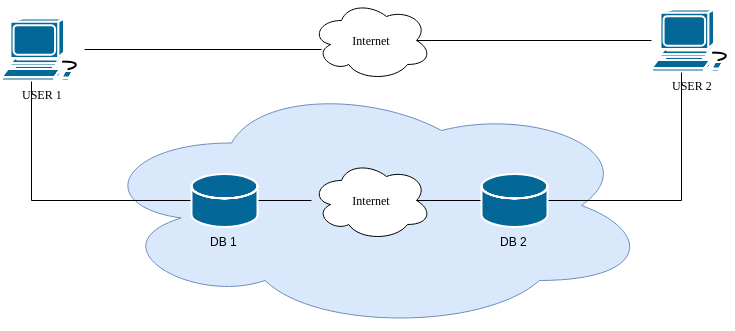
\includegraphics[width=0.8\linewidth]{12/figs/pdv_cloud.png}

    \vspace{2em}

    {\Large Co když dva klienti budou provádět zápisy současně?} \\
    (potenciálně na různé repliky?)
  \end{center}

  Možnosti: \hspace{10pt} Dohodnout se na globálním uspořádání

  \pause
  \hspace{50pt}           \only<2>{Zvolit centrální autoritu, která požadavky seřadí (\emph{leadera})}%
                          \only<3>{\bf Zvolit centrální autoritu, která požadavky seřadí (\emph{leadera})}
\end{frame}

\begin{frame}
  \frametitle{Jak řešit konkurentní požadavky?}
  \begin{center}
    \Large Co když pak požadavek přijme ne-leader?
    \pause

    Přepošle uživateli id nodu, o kterém si myslí, že je leader.
  \end{center}
\end{frame}

\begin{frame}
  \frametitle{Komponenty Raftu}
  %\begin{center}
  {\Large Části raftu:}
    \begin{enumerate}
      \item Volba leader
      \item Replikace logů
    \end{enumerate}
  \pause

  \vspace{2em}\hrule\vspace{2em}

  {\Large Předpokládáme:}

  \begin{itemize}
    \item Fixní konfiguraci známou všem nodům, tzn. počet nodů je fixní a známý všem.
  \end{itemize}
  %\end{center}
\end{frame}

\begin{frame}
  \frametitle{Animace}
  \begin{center}
      \url{http://thesecretlivesofdata.com/raft/}\footnote{Sources at \url{https://github.com/benbjohnson/thesecretlivesofdata}}
  \end{center}
\end{frame}

\begin{frame}
  \frametitle{Volba leadera}

  {\Large \textbf{\faWarning \hspace{3pt} Leader musí mít v DS autoritu!} \hfill Co to znamená?}

  \pause\hspace{20pt} $\rightarrow$ Musí mít důvěru nadpoloviční většiny serverů

  \vspace{2em}\hrule\vspace{2em}

  \textbf{Volba leadera:}
  \begin{enumerate}
    \item Pokud si server myslí, že v systému není leader, chce se jím stát sám.
          \hfill Kdy si myslí, že v systému není leader?
    \pause
    \item Pošle ostatním serverům žádost o to, aby ho respektovali \\
          (zpráva \texttt{RequestVote})

    \item Stane se \texttt{kandidátem}

    \pause
    \item Pokud s tím většina serverů souhlasí, stane se leaderem
  \end{enumerate}
\end{frame}

\begin{frame}
  \frametitle{Volba leadera}

  Přišel Vám \texttt{RequestVote}...
  \begin{center}
    \LARGE Kdy budete \texttt{kandidáta} volit?
  \end{center}

  \pause
  \vspace{2em}
  {\LARGE Dvě podmínky:}
  \begin{itemize}
    \item Požadavek kandidáta musí být aktuální podle ,,logického času``
          \begin{center}
            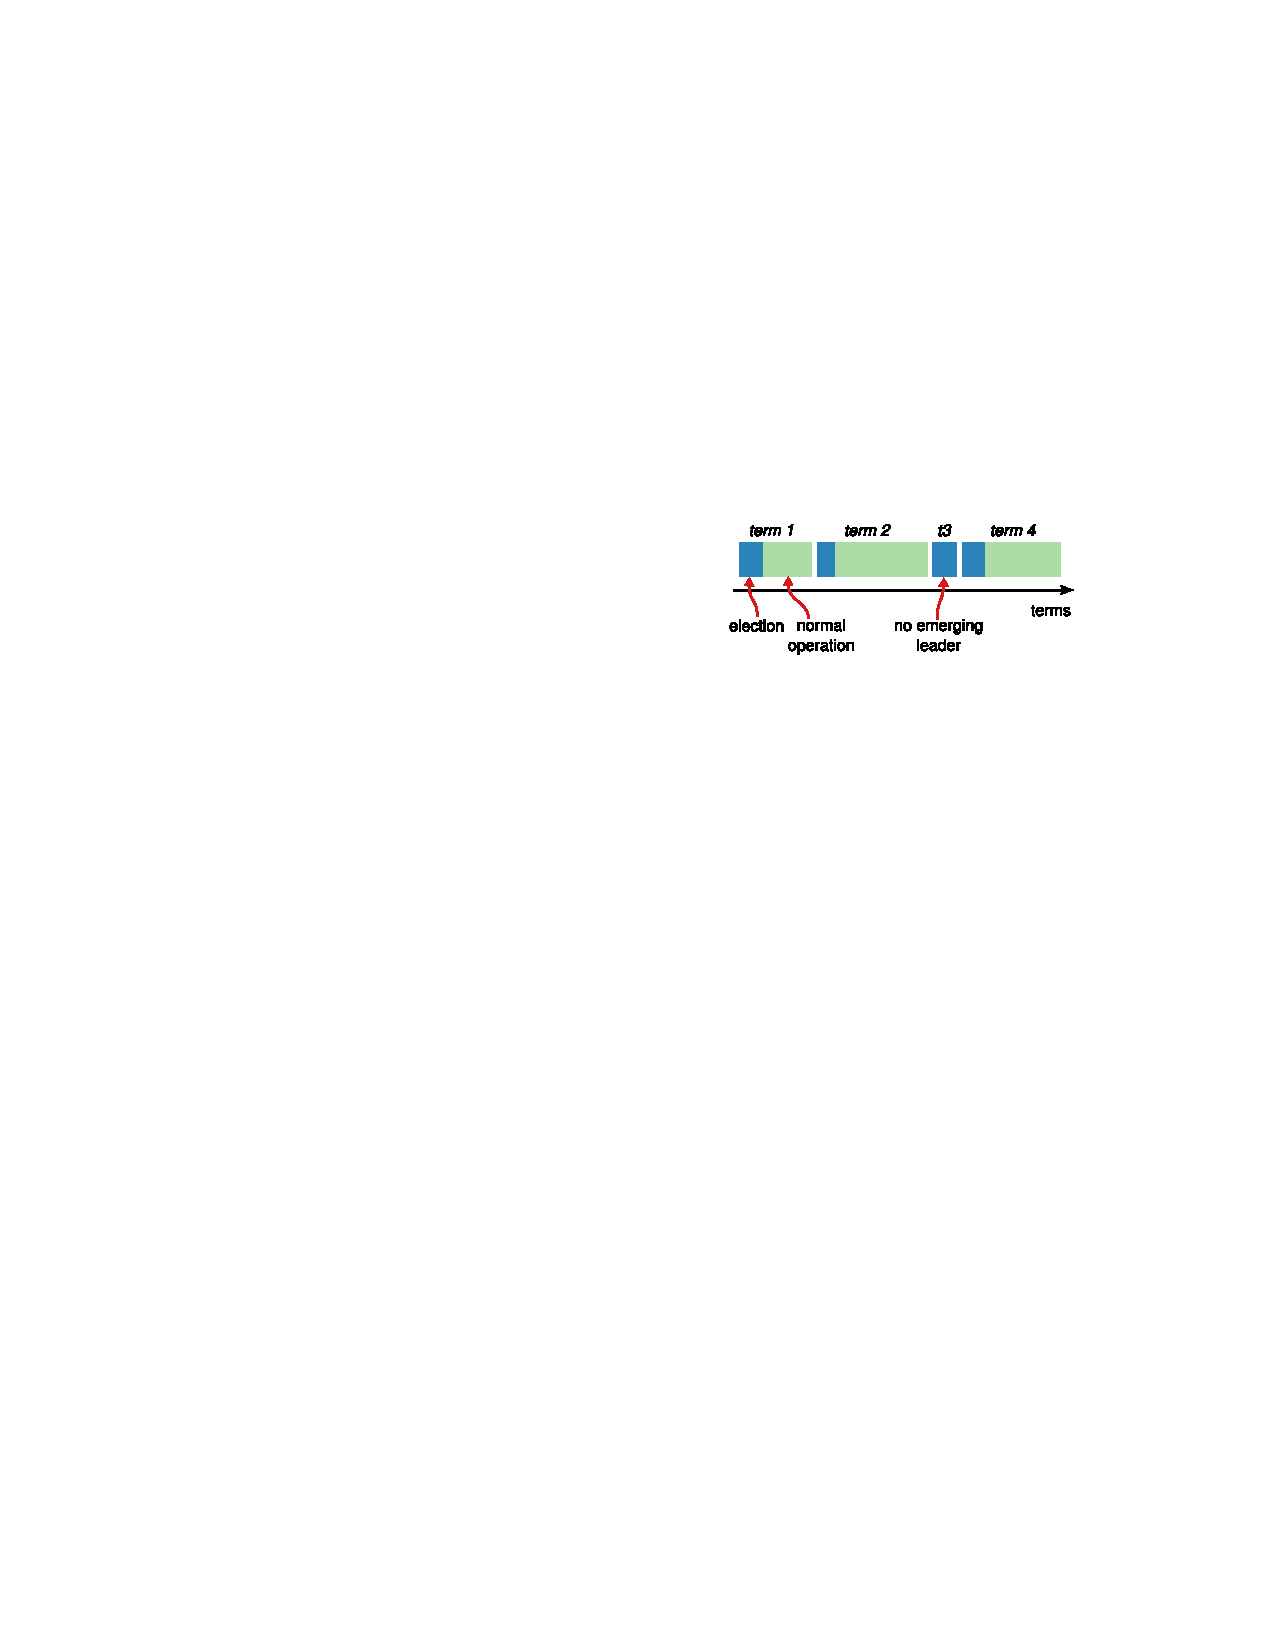
\includegraphics[width=0.5\linewidth]{12/figs/terms.pdf}

            Aktuální \texttt{term} posíláme v každé zprávě.\\
            \texttt{currTerm = max(currTerm, msg.term)}
          \end{center}

    \vspace{1em}

    \pause
    \item Log kandidáta obsahuje všechny potvrzené (\emph{committed}) požadavky

          \pause\hfill To ale nedokážeme zjistit :-(
  \end{itemize}
\end{frame}

\begin{frame}[fragile]
  \frametitle{Log (,,žurnál``)}

  {\large Jediné, co dokážeme zjistit je, jestli je daný log ,,aktuálnější``}

  \hfill
  \begin{minipage}{0.53\linewidth}
    U každého záznamu si držíme \texttt{term}, ve kterém byl zapsaný a jeho pozici (\texttt{index})
  \end{minipage}

  \begin{center}
	  \colorbox{white}{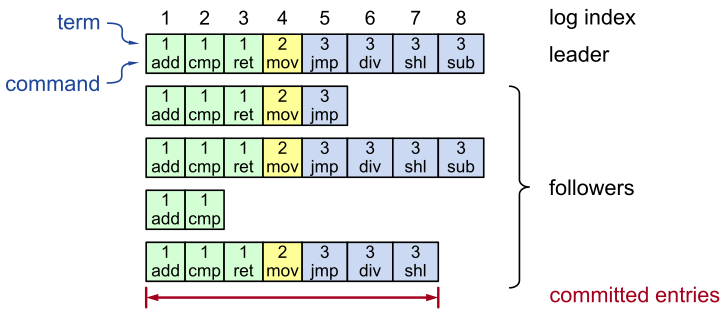
\includegraphics[width=0.7\linewidth]{12/figs/log.png}}
  \end{center}

  \pause\vspace{1em}
  Log \texttt{A} je aktuálnější než \texttt{B} pokud lexikograficky
  \begin{center}
    \footnotesize\texttt{(A[A.last].term, A[A.last].index) > (B[B.last].term, B[B.last].index)}
  \end{center}
\end{frame}

\begin{frame}
  \frametitle{Potvrzování zápisů}

  {\large Zajistí požadavek aktuálnějšího logu kandidáta zvolení leadra se všemi potvrzenými záznamy?}

  \begin{center}
    \LARGE Na kolika serverech musí být záznam zapsaný aby byl potvrzený (commited)?
  \end{center}

  \pause\vspace{2em}\hrule\vspace{2em}

  {\bf \faWarning \hspace{3pt} Stačí nám zapsat záznam na nadpoloviční většinu serverů}
  \begin{itemize}
    \item Pokud by měl být zvolený leaderem server, kterému chybí potvrzený záznam, pak bude mít méně ,,aktuální`` log
  \end{itemize}
\end{frame}

\begin{frame}
  \frametitle{Replikace logu}

  {\large Pro zreplikování záznamu v logu zašle leader zprávu \texttt{AppendEntries} všem followerům}

  \vspace{2em}

  \pause
  {\large Po obdržení potvrzení od většiny serverů považuje zápis za úspěšný}

  \hfill ... a provede změnu v DB a potvrdí úspěch i klientovi

  \pause
  \vspace{3em}\hrule\vspace{1em}
  \begin{center}
    \LARGE Kdy provedou změnu v DB i followeři?
  \end{center}


\end{frame}

\begin{frame}
  \frametitle{Kompletnost logů \hfill \emph{... aneb kdy follower zápis odsouhlasí?}}

  {\Large Pro rekonstrukci stavu z logu, musí být log kompletní!}

  \hfill {Nestačí nám tak shoda na zápisu jednoho prvku do logu}

  \hfill {$\rightarrow$ Musíme se shodnout i na všech předcházejících prvcích}

  \pause\vspace{3em}\hrule\vspace{1em}
  \begin{center}
    \LARGE Co to znamená pro followera?
  \end{center}
\end{frame}

\begin{frame}
  \frametitle{Kompletnost logů \hfill \emph{... aneb kdy follower zápis odsouhlasí?}}

  Ve zprávě \texttt{AppendEntries} posíláme
  \begin{itemize}
    \item Informace o replikovaném záznamu (\texttt{term}, \texttt{index} a obsah záznamu)
  \end{itemize}

  a navíc...
  \begin{itemize}
    \item Informace o záznamu předcházejícím (jeho \texttt{term} a \texttt{index})
  \end{itemize}

  \pause\vspace{3em}\hrule\vspace{1em}
  \begin{center}
    \large Follower zápis odmítne, pokud se na předchozím záznamu neshodne
  \end{center}

  \pause\hfill {\LARGE Ale co pak?} Log musíme nějak doplnit...
\end{frame}

\begin{frame}
  \frametitle{Vlastnosti Raftu}

  \begin{itemize}
    \item V každém \texttt{term}u zvolíme maximálně jednoho leadera. \\[1em]
    % Kolik leaderu může být v systému v jednom okamžiku? CEIL(N/2)

    \pause
    \item Pokud dva logy obsahují stejný záznam (stejný \texttt{term} a \texttt{index}), pak jsou až po \texttt{index} shodné. \\[1em]
     % To je dane 1. pozadavkem ze v jednom termu je max jeden leader, ktery zpracovava pozadavky, a kontrolou predchoziho zaznamu pri append entries
     
    \pause
    \item Pokud někdy klientovi potvrdíme úspěšný zápis, pak nikdy nebude leaderem server, kde tento zápis ještě neproběhl. \\[1em]
  \end{itemize}

  \pause\vspace{2em}\hrule\vspace{1em}

  Kompletní algoritmus je popsaný na:\\
  \url{https://www.cs.princeton.edu/courses/archive/fall16/cos418/papers/raft.pdf}

  \pause\vspace{1em}

  Užitečná je i vizualizace na:\\
  \url{https://raft.github.io/}
\end{frame}

\begin{frame}
  \frametitle{Úpravy raftu - odstranění term inflation}

    Raft je definovaný záměrně co nejjednodušeji, ale pro praxi jsou vyůžívany různá zefektivnění: 

  \uncover<2->{
    \begin{columns}[b]
    \begin{column}{0.5\textwidth}
        Příklad problému: "Term-inflation":
    \end{column}
    \begin{column}{0.5\textwidth}
        \begin{center}
        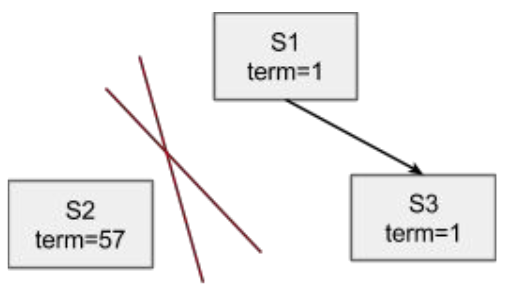
\includegraphics[width=0.9\textwidth]{12/figs/raft_term_inflation.png}
        \end{center}
    \end{column}
    \end{columns}

      \begin{itemize}
        \item Follower odpojený od zbytku systému po každém election timeoutu inkrementuje svůj term. Po zpětném připojení vždy spustí nové volby.
        \uncover<3->{\item Řešení: "Pre-vote", server se stane kandidátem jen pokud má šanci na zvolení\footnote<3->{\href{https://www.openlife.cc/sites/default/files/php_uploads/4-modifications-for-Raft-consensus.pdf}{Paper: Four modifications for the Raft consensus algorithm}}.} 
      \end{itemize}  
    }
\end{frame}

\section{Zadání semestrální práce}
\begin{frame}
  \frametitle{Konsenzus pomocí Raft algoritmu}
 Naimplementujte algoritmus Raft pro replikaci key-value storu

 \vspace{2em}

  Zpracování musí být {\bf distribuované}, procesy si nesahají vzájemně do paměti!


    \pause\vspace{1.5em}

  \begin{tabbing}
      Termín odevzdání je \={\bf 7. 6. 23:59 CET} \\
                          \={(příp. do termínu Vaší zkoušky, pokud byste na ni šli před 7. 6.)}
    \end{tabbing}

\raggedleft Podrobnosti upřesníme.


\end{frame}


% Frame with the feedback QR code
\framefeedback{}

\end{document}
